%%%%%%%%%%%%%%%%%%%%%%%%%%%%%%%%%%%%%%%%%%%%%%%%%%%%%%%%%%%%%%%%%%%%%%%%%%%%%%%%
%%%%%%%%%%%%%%%%%%%%%%%%%%%%%%%%%%%%%%%%%%%%%%%%%%%%%%%%%%%%%%%%%%%%%%%%%%%%%%%%
%%                                                                            %%
%% thesistemplate.tex version 4.21 (2026/02/19)                               %%
%% The LaTeX template file to be used with the aaltothesis.sty (version 4.21) %%
%% style file.                                                                %%
%% This package requires pdfx.sty v. 1.5.84 (2017/05/18) or newer.            %%
%%                                                                            %%
%% This is licensed under the terms of the MIT license below.                 %%
%%                                                                            %%
%% Written by Luis R.J. Costa.                                                %%
%% Currently developed at Teacher services, Learning Services of Aalto        %%
%% University by Luis R.J. Costa since May 2019.                              %%
%%                                                                            %%
%% Copyright 2017-2026 aaltothesis.cls by Luis R.J. Costa,                    %%
%% luis.costa@aalto.fi.                                                       %%
%% Copyright 2017-2018 Swedish translations in aaltothesis.cls by Elisabeth   %%
%% Nyberg and Henrik Wallén henrik.wallen@aalto.fi.                           %%
%% Copyright 2017-2018 Finnish documentation in the template opinnatepohja.tex%%
%% by Perttu Puska, perttu.puska@aalto.fi, and Luis R.J. Costa.               %%
%% Finnish documentation in the template opinnatepohja.tex translated from    %%
%% the English template documentation.                                        %%
%% Copyright 2026 English template thesistemplate.tex by Luis R.J. Costa,     %%
%% Maurice Forget, Henrik Wallén.                                             %%
%% Copyright 2018-2026 Swedish template avhandlingsmall.tex by Henrik Wallen. %%
%%                                                                            %%
%% Permission is hereby granted, free of charge, to any person obtaining a    %%
%% copy of this software and associated documentation files (the "Software"), %%
%% to deal in the Software without restriction, including without limitation  %%
%% the rights to use, copy, modify, merge, publish, distribute, sublicense,   %%
%% and/or sell copies of the Software, and to permit persons to whom the      %%
%% Software is furnished to do so, subject to the following conditions:       %%
%% The above copyright notice and this permission notice shall be included in %%
%% all copies or substantial portions of the Software.                        %%
%% THE SOFTWARE IS PROVIDED "AS IS", WITHOUT WARRANTY OF ANY KIND, EXPRESS OR %%
%% IMPLIED, INCLUDING BUT NOT LIMITED TO THE WARRANTIES OF MERCHANTABILITY,   %%
%% FITNESS FOR A PARTICULAR PURPOSE AND NONINFRINGEMENT. IN NO EVENT SHALL    %%
%% THE AUTHORS OR COPYRIGHT HOLDERS BE LIABLE FOR ANY CLAIM, DAMAGES OR OTHER %%
%% LIABILITY, WHETHER IN AN ACTION OF CONTRACT, TORT OR OTHERWISE, ARISING    %%
%% FROM, OUT OF OR IN CONNECTION WITH THE SOFTWARE OR THE USE OR OTHER        %%
%% DEALINGS IN THE SOFTWARE.                                                  %%
%%                                                                            %%
%%                                                                            %%
%%%%%%%%%%%%%%%%%%%%%%%%%%%%%%%%%%%%%%%%%%%%%%%%%%%%%%%%%%%%%%%%%%%%%%%%%%%%%%%%
%%                                                                            %%
%%                                                                            %%
%% An example for writting your thesis using LaTeX                            %%
%% Original version and development work by Luis Costa, changes to the text   %% 
%% in the Finnish template by Perttu Puska.                                   %%
%% Support for Swedish added 15092014                                         %%
%% PDF/A-b support added on 15092017                                          %%
%% PDF/A-2 support added on 24042018                                          %%
%% Layout design and typesettin changed 15072021                              %%
%%                                                                            %%
%% This example consists of the files                                         %%
%%       thesistemplate.tex (version 4.21) (for text in English)              %%
%%       opinnaytepohja.tex (version 4.21) (for text in Finnish)              %%
%%       avhandlingsmall.tex (version 2.1) (for text in Swedish)              %%
%%       thesistemplate_short.tex (version 4.21) (abridged for text in        %%
%%                                                English)                    %%
%%       aaltothesis.cls (version 4.21)                                       %%
%%       linediagram.pdf (graphics file)                                      %%
%%       curves.pdf      (graphics file)                                      %%
%%       ledspole.jpg    (graphics file)                                      %%
%%                                                                            %%
%%                                                                            %%
%% Typeset in Linux with                                                      %%
%% pdflatex: (recommended method)                                             %%
%%             $ pdflatex thesistemplate                                      %%
%%             $ pdflatex thesistemplate                                      %%
%%                                                                            %%
%%   The result is the file thesistemplate.pdf that is PDF/A compliant, if    %%
%%   you have chosen the proper \documenclass options (see comments below)    %%
%%   and your included graphics files have no problems.                       %%
%%                                                                            %%
%%                                                                            %%
%% Explanatory comments in this example begin with the characters %%, and     %%
%% changes that the user can make with the character %                        %%
%%                                                                            %%
%%%%%%%%%%%%%%%%%%%%%%%%%%%%%%%%%%%%%%%%%%%%%%%%%%%%%%%%%%%%%%%%%%%%%%%%%%%%%%%%
%%%%%%%%%%%%%%%%%%%%%%%%%%%%%%%%%%%%%%%%%%%%%%%%%%%%%%%%%%%%%%%%%%%%%%%%%%%%%%%%
%%
%% WHAT is PDF/A
%%
%% PDF/A is the ISO-standardized version of the pdf. The standard's goal is to
%% ensure that he file is reproducable even after a long time. PDF/A differs
%% from pdf in that it allows only those pdf features that support long-term
%% archiving of a file. For example, PDF/A requires that all used fonts are
%% embedded in the file, whereas a normal pdf can contain only a link to the
%% fonts in the system of the reader of the file. PDF/A also requires, among
%% other things, data on colour definition and the encryption used.
%% Currently three PDF/A standards exist:
%% PDF/A-1: based on PDF 1.4, standard ISO19005-1, published in 2005.
%%          Includes all the requirements essential for long-term archiving.
%% PDF/A-2: based on PDF 1.7, standard ISO19005-2, published in 2011.
%%          In addition to the above, it supports embedding of OpenType fonts,
%%          transparency in the colour definition and digital signatures.
%% PDF/A-3: based on PDF 1.7, standard ISO19005-3, published in 2012.
%%          Differs from the above only in that it allows embedding of files in
%%          any format (e.g., xml, csv, cad, spreadsheet or wordprocessing
%%          formats) into the pdf file.
%% PDF/A-4: based on PDF 2.0, standard ISO19005-4, published in November 2020.
%%
%% PDF/A-1 files are not necessarily PDF/A-2 -compatible and PDF/A-2 are not
%% necessarily PDF/A-1 -compatible.
%% Standards PDF/A-1, PDF/A-2 and PDF/A-3 have two levels:
%% b: (basic) requires that the visual appearance of the document is reliably
%%    reproduceable.
%% a (accessible) in addition to the b-level requirements, specifies how
%%   accessible the pdf file is to assistive software, say, for the physically
%%   impaired.
%% The PDF/A-4 standard does not have additional levels like in the earlier
%% standards.
%% For more details on PDF/A, see, e.g., 
%% https://www.loc.gov/preservation/digital/formats/fdd/fdd000318.shtml or
%% https://www.pdfa.org/resource/iso-19005-pdfa/
%%
%%
%% WHICH PDF/A standard should my thesis conform to?
%%
%% Either to the PDF/A-2b or the PDF/A-1b standard. If all the figures and
%% graphs used in thesis work do not require transparency features, use either
%% PDF/A-1b or PFDF/A-2b. If you have figures with transparency
%% characteristics, use the PDF/A-2b standard. However, drawing applications
%% often use the transparency parameter, setting it to zero, to specify opacity
%% and get the basic 2-D visualisation. As a result, validation of PDF/A-1b
%% will fail. Use PDF/A-2b if PDF/A-1b validation fails.
%% Do not use the PDF/A-3b standard for your thesis.
%% The font to be used are specified in this templatenand they should not be
%% changed. In addition to not adhering to Aalto's visual guidelines, you may
%% have difficulties in producing a PDF/A-compliant PDF.
%%
%%
%% Validate your PDF/A file at https://www.pdf-online.com/osa/validate.aspx
%%
%%
%% WHAT graphics format can I use to produce my PDF/A compliant file?
%%
%% When using pdflatex to compile your work, favour the use of pdf, but you can
%% use the jpg or png format especially for photographs. You will have PDF/A 
%% compliance problems with figures in pdf if the fonts are not embedded in the
%% pdf file.
%% If you choose to use latex to compile your work, the only acceptable file
%% format for your figure is eps. DO NOT use the ps format for your figures.
%%
%% USE one of the following three \documentclass set-ups:
%% * the first when using pdflatex to directly typeset your document in the
%%   chosen pdf/a format for online publishing (centred page layout),
%% * the second for one-sided printing your thesis with the layout (wide left 
%%   margin), or
%% * the third for two-sided printing.
%%
\documentclass[english, 12pt, a4paper, elec, utf8, a-2b, online]{aaltothesis}
%\documentclass[english, 12pt, a4paper, elec, utf8, a-2b, print]{aaltothesis}
%\documentclass[english, 12pt, a4paper, elec, utf8, a-2b, print, twoside]{aaltothesis}

%% Use the following options in the \documentclass macro above:
%% your school: arts, biz, chem, elec, eng, sci
%% the character encoding scheme used by your editor: utf8, latin1
%% thesis language: english, finnish, swedish
%% make an archiveable PDF/A-1b or PDF/A-2b compliant file: a-1b, a-2b
%%                    (with pdflatex, a normal pdf containing metadata is
%%                     produced without the a-*b option)
%% typset for online document or print on paper: online, print
%%        online: typeset in symmetric layout and blue hypertext for online
%%                publishing
%%        print: typeset in a symmetric layout and black hypertext for printing
%%               on paper
%%        twoside: two-sided printing (default is one-sided printing)
%%                 typeset in a wide margin on the binding side of the page and
%%                 black hypertext. Use with print only.
%%

%% FOR USERS OF AMS PACKAGES:
%% * newtxmath used in this template loads amsmath, so
%%   you needn't load it. If you want to use options in amsmath, load it here, 
%%   before \setupthesisfonts below to pass the options to amsmath.
%% * If you want to use amsthm, load it here before \setupthesisfonts to avoid
%%   a clash with newtxmath.
%% * If using amsmath with options and you want to use amsthm, load amsthms
%%   after amsmath, as described in the amsthm documentation.
%% * Don't use amsbsym or amsfonts. The symbols [and macros] there are defined in
%%   newtxmath and so clash if used.
%\usepackage[options]{amsmath}
%\usepackage{amsthm}

%% DO NOT MOVE OR REMOVE \setupthesisfonts
\setupthesisfonts

%%
%% Add here the packges you need
%%
\usepackage{graphicx}
\usepackage[utf8]{inputenc} 
\usepackage[T1]{fontenc}
\usepackage{xspace}
\usepackage{booktabs}
%% For tables that span multiple pages; used to split a paraphrasing example in
%% the appendix. If you don't need it, remove it.
\usepackage{longtable}

%% A package for generating Creative Commons copyright terms. If you don't use
%% the CC copyright terms, remove it, since otherwise undesired information may
%% be added to this document's metadata.
\usepackage[type={CC}, modifier={by-nc-sa}, version={4.0}]{doclicense}
%% Find below three examples for typesetting the CC license notice.

% Use listings package to insert code block. Also define code block style.
\usepackage{listings}
\renewcommand{\lstlistingname}{Code Block}
% For color
\usepackage{xcolor}

\lstdefinestyle{mystyle}{
    backgroundcolor=\color{gray!10},
    commentstyle=\color{green!50!black},
    keywordstyle=\color{blue},
    stringstyle=\color{blue},
    basicstyle=\ttfamily\footnotesize,
    breakatwhitespace=false,
    breaklines=true,
    captionpos=b,
    keepspaces=true,
    showspaces=false,
    showstringspaces=false,
    showtabs=false,
    tabsize=2,
    frame=single
}

\lstdefinelanguage{json}{
    basicstyle=\ttfamily\footnotesize,
    showstringspaces=false,
    breaklines=true,
    frame=single,
    literate=
     *{0}{{{\color{blue}0}}}{1}
      {1}{{{\color{blue}1}}}{1}
      {2}{{{\color{blue}2}}}{1}
      {3}{{{\color{blue}3}}}{1}
      {4}{{{\color{blue}4}}}{1}
      {5}{{{\color{blue}5}}}{1}
      {6}{{{\color{blue}6}}}{1}
      {7}{{{\color{blue}7}}}{1}
      {8}{{{\color{blue}8}}}{1}
      {9}{{{\color{blue}9}}}{1}
      {:}{{{\color{black}{:}}}}{1}
      {,}{{{\color{black}{,}}}}{1}
      {\{}{{{\color{blue}{\{}}}}{1}
      {\}}{{{\color{blue}{\}}}}}{1}
      {[}{{{\color{blue}{[}}}}{1}
      {]}{{{\color{blue}{]}}}}{1},
}

\lstset{style=mystyle}

%% Edit to conform to your degree programme
%% Capitalise the words in the name of the degree programme: it's a name
\degreeprogram{Computer, Communication and Information Sciences}
%%

%% Your major
%%
\major{Computer Science}
%%

%% Choose one of the three below
%%
%\univdegree{BSc}
\univdegree{MSc}
%\univdegree{Lic}
%%

%% Your name (self explanatory...)
%%
\thesisauthor{Han Le}
%%

%% Your thesis title and possible subtitle comes here and possibly, again,
%% together with the Finnish or Swedish abstract. Do not hyphenate the title
%% (and subtitle), and avoid writing too long a title. Should LaTeX typeset a
%% long title (and/or subtitle) unsatisfactorily, you might have to force a
%% linebreak using the \\ control characters. In this case...
%% * Remember, the title should not be hyphenated!
%% * A possible 'and' in the title should not be the last word in the line; it
%%   begins the next line.
%% * Specify the title (and/or subtitle) again without the linebreak characters
%%   in the optional argument in box brackets. This is done because the title
%%   is part of the metadata in the pdf/a file, and the metadata cannot contain
%%   linebreaks.
%%
\thesistitle{UniMCP: A Standardized Model Context Protocol Integration Framework for  GenAI Production System in University}
%\thesistitle[Title of the thesis]{Title of\\ the thesis}
%%
%% Either remove or leave \thesissubtitle{} empty if you don't use it
%%
\thesissubtitle{Case Study: Aalto AI Assistant}
%\thesissubtitle[Subtitle of the thesis]{Subtitle of\\ the thesis}
%\thesissubtitle{}

%%
\place{Espoo}
%%

%% The date for the bachelor's thesis is the day it is presented
%%
\date{19 February 2026}
%%

%% Thesis supervisor
%% Note the "\" character in the title after the period and before the space
%% and the following character string.
%% This is because the period is not the end of a sentence after which a
%% slightly longer space follows, but what is desired is a regular interword
%% space.
%%
\supervisor{Prof.\ Bo Zhao}
%%

%% Advisor(s)---two at the most---of the thesis. Check with your supervisor how
%% many official advisors you can have.
%%
\advisor{Joonas Uusnäkki (M.Sc.)}
\advisor{Zheyue Tan (M.Sc.)}
%%

%% If you do your thesis work in a company or other institution, give the name
%% of the company or instution here. Otherwise, leave the macro empty, comment
%% it out, or remove it. This will remove this field from the abstract page.
%%
\collaborativepartner{Aalto University}
%%

%% Aaltologo: syntax:
%% \uselogo{?|!|'|aalto?|aalto!|aalto'|<empty>}
%% The logo language is set to be the same as the thesis language.
%%
%\uselogo{?}
%\uselogo{!}
%\uselogo{'}
%\uselogo{aalto?}
\uselogo{aalto!}
%\uselogo{aalto'}
%\uselogo{}
% Preamble to the framework name
\newcommand{\UniMCP}{\textbf{UniMCP}\xspace}
\newcommand{\aitutor}{\text{AI Tutor}\xspace}
\newcommand{\aaltoai}{\text{Aalto AI Assistant}\xspace}
\newcommand{\aalto}{\text{Aalto University}\xspace}
%%%%%%%%%%%%%%%%%%               COPYRIGHT TEXT               %%%%%%%%%%%%%%%%%%
%%%%%%%%%%%%%%%%%%%%%%%%%%%%%%%%%%%%%%%%%%%%%%%%%%%%%%%%%%%%%%%%%%%%%%%%%%%%%%%%

%% Copyright of a work is with the creator/author of the work regardless of
%% whether the copyright mark is explicitly in the work or not. You may, if you
%% wish---we encourage you to do so---publish your work under a Creative
%% Commons license (see creativecommons.org), in which case the license text
%% must be visible in the work. Write here the copyright text you want using the
%% macro \copyrighttext, which writes the text into the metadata of the pdf file
%% as well.
%%
%% Syntax:
%% \copyrigthtext{metadata text}{text visible on the page}
%%
%% CHOOSE ONE OF THE COPYRIGHT NOTICE STYLES BELOW.
%% IF USING THE CC TERMS, CHOOSE THE LICENSE YOU WANT TO USE.
%% The different CC licenses are listed at 
%% https://creativecommons.org/about/cclicenses/.
%% If you use the icons from the doclicense.sty package, add the package above
%% (\usepackage{doclicense}).
%% IMPORTANT NOTE!! Manually write the CC text in the \copyrighttext metadata
%% text field.
%%
%% NOTE: In the macros below, the text written in the metadata must have a
%% \noexpand macro before the \copyright special character. When not in pdf/a
%% mode (i.e. a-1b or a-2b are not specified in \documentclass), two \noexpands
%% are required in the metadata text to correctly render the copyright mark in
%% the pdf metadata. In pdf/a mode one \noexpand suffices.
%%
%% EXAMPLE OF PLAIN COPYRIGHT TEXT
%% The macros \copyright and \year below must be separated by the \ character 
%% (space chacter) from the text that follows. The macros in the argument of the
%% \copyrighttext macro automatically insert the year and the author's name.
%% (Note! \ThesisAuthor is an internal macro of the aaltothesis.cls class file).
%%
%\copyrighttext{Copyright \noexpand\textcopyright\ \number\year\ \ThesisAuthor}
%{Copyright \textcopyright{} \number\year{} \ThesisAuthor}
%%
%% Of course, the same text could have simply been written as
%% \copyrighttext{Copyright \noexpand\copyright\ 2018 Eddie Engineer}
%% {Copyright \copyright{} 2022 Eddie Engineer}
%%
%% EXAMPLES OF CC LICENSE: different ways to display the same license
%% 1. A simple Creative Commons license text with a link to the copyright notice:
%\copyrighttext{\noexpand\textcopyright\ \number\year. This work is 
%	licensed under a CC BY-NC-SA 4.0 license.}{\textcopyright{} 
%	\number\year. This work is licensed under a 
%	\href{https://creativecommons.org/licenses/by-nc-nd/4.0/}{CC BY-NC-SA 4.0} 
%	license.}
%
%% To get the URL of the license of your choice, go to 
%% https://creativecommons.org/about/cclicenses/, click on the chosen license
%% you want to use, and copy-and-paste the URL in the macro \href above.
%%
%% 2. A short Creative Commons license text containing the respective CC icons
%% (requires the package doclicense.sty to be added in the preamble as done
%% above) and a link to the corresponding Creative Commons license webpage (see
%% the doclicense package documentation for other license icons):
%\copyrighttext{\noexpand\textcopyright\ \number\year. This work is licensed
%	under a CC BY-NC-SA 4.0 license.}{
%	\parbox{95mm}{\noindent\textcopyright\ \number\year. \doclicenseText} 
%	\hspace{1em}\parbox{35mm}{\doclicenseImage}
%}
%%
%% 3. An expanded Creative Commons license text containing the respective CC
%% icons text and as generated by the doclicense.sty package (the license is set
%% via package options in \usepackage[options]{doclicense} above; see the
%% doclicense package documentation for other license texts and icons):
\copyrighttext{\noexpand\textcopyright\ \number\year. This work is 
	licensed under a Creative Commons "Attribution-NonCommercial-ShareAlike 4.0 
	International" (BY-NC-SA 4.0) license.}{\noindent\textcopyright\ \number
	\year \ \doclicenseThis}
%%%%%%%%%%%%%%%%%%%%%%%%%%%%%%%%%%%%%%%%%%%%%%%%%%%%%%%%%%%%%%%%%%%%%%%%%%%%%%%%


%% The English abstract:
%% All the details (name, title, etc.) on the abstract page appear as specified
%% above.
%% Thesis keywords:
%% Note! The keywords are separated using the \spc macro.
%%
\keywords{For keywords choose concepts that are central to your 
thesis. Keywords are written in lowercase with the exception of certain
abbreviations and proper nouns. E.g.\spc artificial intelligence\spc generative artificial intelligence\spc large language model}
%%

%% The abstract text. This text in one paragraph is included in the metadata of
%% the pdf file as well as the abstract page. To have paragraphs in your
%% abstract rewrite it in the abstarct environment as described below.
%%
\thesisabstract{%
The abstract is a short description of the essential contents of the thesis
usually in one paragraph: what was studied and how and what were the main
findings. For a Finnish thesis, the abstract should be written in both Finnish
and English; for a Swedish thesis, in Swedish and English. The abstracts for
English theses written by Finnish or Swedish speakers should be written in
English and either in Finnish or in Swedish, depending on the student’s language
of basic education. Students educated in languages other than Finnish or Swedish
write the abstract only in English. Students may include a second or third
abstract in their native language, if they wish. 
The abstract text of this thesis is written on the readable abstract page as
well as into the pdf file's metadata via the thesisabstract macro (see the 
comment in the TeX file). Write here the text that goes into the metadata. The 
metadata cannot contain special characters, linebreak or paragraph break 
characters, so these must not be used here. If your abstract does not contain 
special characters and it does not require paragraphs, you may take advantage of
the abstracttext macro (see the comment in the TeX file below). Otherwise, the 
metadata abstract text must be identical to the text on the abstract page.
}

%% You can prevent LaTeX from writing into the xmpdata file (it contains all the 
%% metadata to be written into the pdf file) by setting the writexmpdata switch
%% to 'false'. This allows you to write the metadata in the correct format
%% directly into the file thesistemplate.xmpdata.
%\setboolean{writexmpdatafile}{false}


%% All that is printed on paper starts here
%%
\begin{document}

%% Create the coverpage
%%
\makecoverpage

%% Typeset the copyright text.
%% If you wish, you may leave out the copyright text from the human-readable
%% page of the pdf file. This may seem like a attractive idea for the printed
%% document especially if "Copyright (c) yyyy Eddie Engineer" is the only text
%% on the page. However, the recommendation is to print this copyright text.
%%
\makecopyrightpage

\clearpage
%% Note that when writing your thesis in English, place the English abstract
%% first followed by the possible Finnish or Swedish abstract.

%% Abstract text
%% All the details (name, title, etc.) on the abstract page appear as specified
%% above. Add your abstarct text with paragraphs here to have paragraphs in the
%% visible abstract page. Nonetheless, write the abstarct text without
%% paragraphs in the macro \thesismacro so that it is added to the metadata as
%% well.
%%
\begin{abstractpage}[english]

  The abstract text of this thesis is written on the readable abstract page as
  well as into the pdf file's metadata via the \verb+\thesisabstract+ macro
  (see comment in this \TeX{} file above). The metadata cannot contain special 
  characters, word hyphenations, linebreak or paragraph break characters, so 
  these must not be used there. Write here the text that goes onto the readable 
  abstract page. You can have special characters, linebreaks, and paragraphs 
  here. Otherwise, this abstract text must be identical to the metadata abstract 
  text.
  
  If your abstract does not contain special characters and it does not require
  paragraphs, you may take advantage of the \verb+\abstracttext+ macro (see the
  comment in this \TeX{} file below).
\end{abstractpage}

%% The text in the \thesisabstract macro is stored in the macro \abstractext, so
%% you can use the text metadata abstract directly as follows:
%%
%\begin{abstractpage}[english]
%	\abstracttext{}
%\end{abstractpage}

%% Force a new page so that the possible Finnish or Swedish abstract does not
%% begin on the same page
%%
\newpage

%% Force new page so that the Swedish abstract starts from a new page
\newpage

\dothesispagenumbering{}

%% Preface
%%
%% This section is optional. Remove it if you do not want a preface.
\mysection{Preface}
%\mysection{Esipuhe}
I want to thank Professor Bo Zhao and my advisors Joonas Uusnäkki and Zheyue Tan for their guidance.

\vspace{5cm}
Otaniemi, 28 September 2026\\

\vspace{5mm}
{\hfill Han Le \hspace{1cm}}

%% Force a new page after the preface
%%
\newpage


%% Table of contents. 
%%
\thesistableofcontents
%% An example of an ordered (numbered) list with the default numbering.
%\begin{enumerate}
	%\item \label{list:intro} Introduction (research objectives and questions)
	%\item Literature review (research made earlier in this area)
	%\item Research material and methods
	%\item Results / Findings
	%\item Discussion
	%\item \label{list:summary} Summary / Conclusions
	%\item References
%\end{enumerate}

%% Symbols and abbreviations
\mysection{Symbols and abbreviations}

\subsection*{Symbols}

\begin{tabular}{ll}

\end{tabular}

\subsection*{Operators}

\begin{tabular}{ll}

\end{tabular}

\subsection*{Abbreviations}

\begin{tabular}{ll}
AI          & Artificial Intelligence \\
MCP         & Model Context Protocol \\
LLM         & Large Language Model \\

\end{tabular}


%% \clearpage is similar to \newpage, but it also flushes the floats (figures
%% and tables).
%%
\cleardoublepage

%% Text body begins.
%%
% ============================================================
\section{Introduction}
\label{chap:intro}
% ============================================================
%% Leave page number of the first page empty
%% 
\thispagestyle{empty}

Large language models (LLMs) are rapidly integrated into production systems and connected to external tools, data sources, and services. 
This adoption has brought about the new paradigm of agentic systems—these modern autonomous software systems utilize LLMs and other machine learning algorithms to perceive the user's prompt, decide on the best approach, take actions using available tools, and learn from the results.
This paradigm shift of AI's capabilities from passive text generation to active tool use demands a robust, standardized framework in how AI is deployed and how to control AI's communication with external resources securely.

As a result, the Model Context Protocol (MCP), introduced by Anthropic in November 2024, has emerged as a middleware layer that standardizes how AI agents connect with external systems and interact with the world beyond the training data of their LLMs \cite{anthropic_mcp_intro}.
MCP introduces an interface through which LLMs can find, invoke, and interact with external tools, databases, and APIs through a unified communication layer based on the JSON-RPC protocol \cite{hou2025landscape}.
From the point of view of scalability, MCP aims to solve the bottleneck of the \textit{N$\times$M integration problem}, which occurs when there are \textit{M} number of AI models that need to connect to \textit{N} external tools or data sources \cite{ray2025survey}. 
Without MCP, each model requires a bespoke integration for each external tool or data source that it interacts with, turning this into the \textit{N$\times$M integration problem}. 
Thanks to MCP, the AI model's reasoning is separated from tool execution, which enables a robust, scalable architecture in which new tools can be added without modifying the underlying agentic pipeline. 
As a result, MCP are rapidly adopted by industry vendors within months of its release, including Google, GitHub, and Figma.
For example, Google Calendar has offered an MCP server that allows AI agents to access Google Calendar data and acts as a customized AI assistant to check availability or create and update events \cite{google_calendar_mcp}.
GitHub MCP server allows AI assistants to perform common GitHub operations such as read code repositories, manage issues and pull requests, and retrieve file contents \cite{github-mcp-server}.
By June 2026, the MCP ecosystem is estimated to have grown to over 17,000 MCP servers, ranging from community-developed to enterprise-grade MCP servers \cite{glama_mcp_servers_2026}. 

% problems
However, at the same time, this rapid adoption of MCP has exposed critical gaps in the security and infrastructure to connect AI agents to external resources. 
Currently, MCP provides only minimal built-in security guaranties by enforcing basic JSON schema validation and request traceability.
It does not offer native support for authentication or confidentiality; therefore, the burden of securing tool interactions falls largely on individual developers \cite{yan2025mcpmisuse}. 
This has led to multiple cybersecurity threats, including malicious prompt injection and MCP servers, cryptographic misuse, and insufficient access control mechanisms in the MCP ecosystem. 
Furthermore, deploying MCP at organizational scale introduces additional challenges in scalability, multi-tenancy, and trust. 
This issue is especially critical in the production systems of higher education institutions such as universities, where sensitive personal data, identity-bound services, and critical workflows are involved. 

% research questions and the sub-problems in the line of inquiry
The thesis addresses the research gap by proposing an MCP integration framework for GenAI systems in university contexts.
The framework is developed and validated through a case for Aalto AI Assistant \cite{aalto_ai_assistant}, a chat-based assistant tool for internal users at Aalto University based in Espoo, Finland.
Specifically, we integrate into Aalto AI Assistant's production system a service called AI Tutor.

This thesis is carried out as a project at Aalto University IT Services (Aalto ITS), and Aalto AI Assistant serves as the primary case study, providing a real production environment in which to design, implement, and evaluate the proposed \UniMCP, an MCP Integration Framework.

The thesis focuses on answering two main research questions: 
\begin{enumerate}
    \item How can MCP be securely integrated into a GenAI production system for university use?
    \item How can a scalable MCP framework be designed and implemented within a university's GenAI production system?
    %\item Is it possible to evaluate the trustworthiness of an MCP agent operating within a university's GenAI system?
\end{enumerate}

% the scope and constraints of the study along with the goals and main concepts involved.
To answer these questions, this thesis studies the MCP architecture, identifies security and scalability challenges associated with MCP-based integration, and designs an MCP integration framework for university contexts. 
The main contribution of the thesis is \UniMCP, a practical framework for integrating MCP into GenAI production systems in university environments. 
The framework is named \UniMCP as the thesis project is conducted at Aalto University IT Services, and its design is motivated by the systems, environment, and use cases of Aalto University. 
The framework is developed and evaluated through a case study of Aalto AI Assistant \cite{aalto_ai_assistant}, a GenAI-based assistant tool for internal users at Aalto University in Espoo, Finland. 

As a proof of concept, the \UniMCP is validated through the development of \aitutor, a student-facing AI agent embedded in Aalto AI Assistant, to validate the proposed framework in a concrete university use case. The evaluation focuses on integration security, scalability, and trustworthiness, corresponding to the three research questions. More broadly, the thesis provides lessons for universities seeking to adopt tool-using GenAI assistants while maintaining security, scalability, privacy, and reliability.

% What each chapter in the thesis is about


%% In a thesis, every section/chapter starts a new page, hence the \clearpage

\clearpage
% ============================================================
\section{Background of MCP}
\label{chap:mcp_background}
% ============================================================
% what this chapter is about
This chapter studies the background, core architectural components, and workflow of Model Context Protocol (MCP). 
In addition, current landscape of the MCP ecosystem is analyzed by studying MCP adoption and use cases relevant to the field of higher education.

\subsection{Overview of Model Context Protocol}
% Explain what MCP is.
It is important to first understand the big picture of Model Context Protocol (MCP).
Introduced by Anthropic in November 2024, MCP is an open-source standard that defines how an AI application exchanges context with external tools and data sources through a uniform interface, rather than through bespoke, tool-specific integration code \cite{anthropic_mcp_intro}.
% Why it was introduced
Hence, MCP can reduce custom code for every AI-to-data connection and solve the \textit{N$\times$M integration problem} \cite{ray2025survey}. 

MCP follows a host-client-server architecture illustrated in Fig. \ref{fig:mcp_architecture} \cite{mcp_architecture}. 
A host is an AI application, such as Claude Desktop, that embeds one or more MCP clients.
Each MCP client maintains a connection to a single MCP server and uses contexts and capabilities from that MCP server. 
Contexts are the stream of information that flows into the language model via the server, such as external data or files. 
Capabilities are the features a server declares to the client that it can provide during connection setup, such as writing a file or running a query.
In-depth details of three key participants in MCP—host, client, and server—are discussed further in Section \ref{sec:mcp_components}.

\begin{figure}[h]
    \centering
    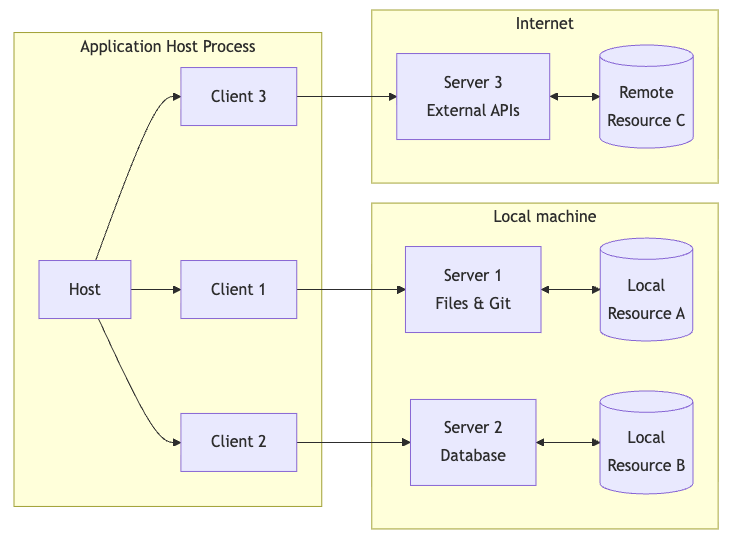
\includegraphics[width=0.8\textwidth]{figures/mcp_architecture.png}
    \caption{MCP architecture adopts a host-client-server pattern where each host can run several clients. Remote MCP servers use Streamable HTTP transport and serve many clients simultaneously, while local MCP servers use the STDIO (Standard Input/Output) transport on a local machine and typically serve one client. The figure is adapted from the official MCP documentation \cite{mcp_architecture}.}
    \label{fig:mcp_architecture}
\end{figure}

An important concept in MCP is primitives. 
They are the fundamental building blocks for adding contexts to the language model and enrich interactions between client, server, and language model. 
MCP specification defines three primitives that a server can expose to a client as follow: 
\begin{enumerate}
    \item Tools: Tools are functions that the LLM can invoke to take action, for example, API calls, database queries, and information search. 
    \item Resources: Resources are data that inject contextual data into the model such as API responses, databases, and file contents. 
    \item Prompts: Prompts are reusable instructions that standardize how users and clients interact with the LLMs.
\end{enumerate}

According to the official documentation of MCP \cite{mcp_architecture}, it has two layers: (1) a data layer that implements the JSON-RPC 2.0 based exchange protocol, lifecycle management, and the server and client features described above, 
and (2) a transport layer that defines the connection-establishment, message-framing, and authorization mechanisms specific to each transport, such as STDIO or Streamable HTTP.
Conceptually, the data layer is the inner layer, while the transport layer is the outer layer.
This thesis focuses on the data layer of MCP, which is studied further in Section \ref{sec:data_layer}. 

% ============================================================
\subsection{MCP Core Components}
\label{sec:mcp_components}
% ============================================================
This section studies the three key components of an end-to-end MCP architecture: host, client, and server.

\subsubsection{MCP Host}
In MCP architecture, MCP host is an AI application that the end user interacts with and coordinates and manages one or multiple MCP clients \cite{mcp_architecture}.
Architecturally, the host acts as the container and coordinator for all MCP
activity within the application: it creates and manages client instances,
controls their connection permissions and lifecycle, enforces security policies
and consent requirements, and handles user authorization
decisions~\cite{mcpspec2026}.
Because a single host can connect to multiple MCP servers simultaneously, it is
also responsible for aggregating the tool, resource, and prompt catalogues
exposed by all connected servers into a unified context presented to the
underlying LLM.
The host is therefore the component that decides what information is visible to
the model and mediates between the model's requests to invoke tools and the
policies governing which invocations are permitted.
Examples of MCP hosts include chat-based GenAI applications such as Claude and ChatGPT, IDE-integrated assistants such as VS Code with GitHub Copilot and Cursor. 
In the context of this thesis, the Aalto AI Assistant platform \cite{aalto_ai_assistant} acts as the MCP host for the \aitutor proof of concept described in Chapter \ref{chap:implementation}. 

\subsubsection{MCP Client}
\label{sec:mcp-client}
The MCP client is embedded inside the MCP host and maintains the actual connection to a single MCP server. 
The host instantiates one client for every server it connects to, so a host that uses three different MCP servers will maintain three separate, isolated client sessions. 

At session initialization, the client performs the capability-negotiation handshake described in on the host's behalf, and for the remainder of the session it is the channel through which the host forwards tool invocations, resource requests, and prompt requests to the server, and through which the server's responses and notifications are relayed back to the host \cite{mcpclient2026}. 
Because each client-server pair forms its own isolated session, permissions, policies, and protocol state negotiated with one server do not leak into a different client's session with a different server.

\subsubsection{MCP Server}
\label{sec:mcp-server}

An MCP server is a program that exposes capabilities---tools, resources, and
prompts---to MCP clients through the standardized MCP primitives.
Servers operate independently with focused responsibilities, and each server
maintains its own capability set that is negotiated with the client during
session initialization~\cite{mcpspec2026}.
MCP servers can be deployed in two modes that differ substantially in their
operational and security characteristics.

\paragraph{Local MCP Server.}
A local MCP server runs as a subprocess on the same machine as the host and
communicates with its client exclusively through standard input and output (the
STDIO transport)~\cite{mcpspec2026}.
Because the server process is spawned and supervised by the host, its source
code or binary is present on the user's machine and can in principle be
inspected, version-pinned, or sandboxed by the operating system before
execution.
This makes local servers well suited for resources that are inherently local to
the user's environment---a filesystem, a local Git repository, or an
on-premises database---and they are the deployment mode adopted by most
reference implementations published by the MCP project.
Their primary limitation is scalability: a STDIO server maintains a
one-to-one relationship with its client and serves a single user session at a
time, making the local mode unsuitable for an organization-wide system serving
many concurrent users simultaneously.

\paragraph{Remote MCP Server.}
A remote MCP server is hosted on infrastructure separate from the user's
machine and communicates with the MCP client over a network connection, most
commonly using the Streamable HTTP transport~\cite{mcpspec2026}.
Streamable HTTP exposes the server through a single unified HTTP endpoint over
which the client can send requests and receive both standard HTTP responses and
streamed server notifications, enabling efficient bidirectional communication
without requiring a persistent socket connection.
Unlike a local server, a single remote MCP server can serve many clients
concurrently---the deployment mode required for an organization-wide GenAI
assistant serving many simultaneous users.
This scalability advantage comes at the cost of introducing authentication,
authorization, and multi-tenancy concerns that the base MCP specification
delegates to server implementers, as discussed further in
Chapter \ref{chap:challenges}.

Remote MCP Server can be connected with Streamable HTTP. 
This is a transport protocol used for the Model Context Protocol (MCP) that enables AI agents to communicate with remote services using a single, unified HTTP endpoint. 

% ============================================================
\subsection{Data layer of MCP}
\label{sec:data_layer}
% ============================================================
The foundation of MCP's data layer is JSON-RPC 2.0 \cite{jsonrpc2020}, a stateless Remote Procedure Call (RPC) that enables structured communication between client and server using JSON format.
JSON-RPC is a JSON-based wire protocol for RPC \cite{jsonrpc2020}.

On top of the underlying JSON-RPC 2.0 protocol, MCP incorporates a stateful session protocol. 
The data layer protocol defines the ways developers can share context from MCP servers to MCP clients.
MCP requires lifecycle management to negotiate the capabilities that both the client and server support before any tool, resource, or prompt can be used. 
In the example in Code Block \ref{lst:mcp_example}, a session begins with an initialization handshake in which the client and server declare their protocol version and capabilities. for example, whether the server supports resource subscriptions or the client supports sampling.
Only capabilities declared during this exchange may be used for the remainder of the session, and the session ends with an explicit termination step.
 
\begin{lstlisting}[language=JSON, caption={Example MCP initialization in life cycle management. The code is adopted from MCP official documentation \cite{mcp}.}, label={lst:mcp_example}]
{
  "jsonrpc": "2.0",
  "id": 1,
  "method": "initialize",
  "params": {
    "protocolVersion": "2025-06-18",
    "capabilities": {
      "elicitation": {}
    },
    "clientInfo": {
      "name": "example-client",
      "version": "1.0.0"
    }
  }
}
\end{lstlisting}

% How it supports tool-using AI systems.

The separation between a data layer and a transport layer is what allows the same JSON-RPC semantics to run unchanged over a local subprocess pipe or a remote HTTPS endpoint, which is the distinction elaborated further in Section \ref{sec:mcp_workflow}.

% ============================================================
\subsection{MCP Workflow}
\label{sec:mcp_workflow}
% ============================================================

An end-to-end MCP interaction proceeds through four sequential
stages~\cite{mcpspec2026}.

In the \textbf{initialization} stage, the host creates a client and directs it
to connect to the target server.
The client sends an initialization request carrying its protocol version and
supported capabilities; the server responds with its own protocol version and
capabilities.
Both parties must agree on a compatible protocol version before proceeding, and
only capabilities declared during this handshake may be used for the remainder
of the session.

In the \textbf{discovery} stage, the client requests the catalogues of tools,
resources, and prompts currently exposed by the server.
The host incorporates the names, descriptions, and input schemas of these
primitives into the context provided to the LLM, so the model can reason about
which capabilities are available and how to invoke them.
Only the declared interface of each primitive is visible to the model; the
server's internal implementation is never exposed.

During the \textbf{operation} stage, a user- or model-initiated action causes
the host to direct the client to send a request to the server---most commonly
a tool invocation.
The server executes the corresponding handler and returns a structured response;
the client relays this response to the host, which integrates it into the
conversation context and passes it to the LLM for further reasoning.
This request-response loop may repeat any number of times within a single
session.
In addition to client-initiated requests, the server may independently push
resource-update notifications to the client, and the server may initiate
sampling requests that ask the host LLM to generate content, enabling
bidirectional, dynamic interactions beyond the simple request-response pattern.

The session concludes with a \textbf{termination} stage in which either party
sends an explicit close notification and the underlying transport connection is
released.

In the AI Tutor proof of concept (Chapter~\ref{chap:implementation}), a session
initializes when a student opens AI Tutor inside Aalto AI Assistant; the
operation stage carries the transcript-retrieval and course-recommendation tool
calls described in Section~\ref{sec:aitutor-use-cases}; and the session
terminates when the student closes the conversation.

\subsection{Current Ecosystem of MCP}
%The emergence of Gen AI tools in recent year has accelerated a new paradigm of interactive and tailored AI agents that focus on a specific, tailored application. FastMCP’s OpenAPI converter has become one of the most popular tools for auto-generating MCP servers from REST APIs.

\label{sec:mcp-ecosystem}
Since the public release of MCP in November 2024, a large and rapidly growing ecosystem of tooling, server implementations, and client integrations has formed around the technology of MCP.
On the tooling side, libraries such as FastMCP have substantially lowered the barrier to creating new MCP servers: FastMCP's OpenAPI converter \cite{fastmcp_openapi2026} can automatically generate a working MCP server from an existing REST API specification, so that organizations with established API infrastructure can expose their services to LLM agents without writing MCP-specific server
code from scratch.
MCP's official SDK support now spans multiple common programming languages, including TypeScript, Python, Java, and C\#, reflecting the protocol's uptake across diverse development ecosystems.

On the adoption side, industry growth has been rapid.
Major technology companies including Microsoft,
Google, and Bloomberg have published accounts of MCP adoption for
engineering and productivity workflows.
Public server registries track the resulting expansion: the Glama AI registry,
which indexes community-contributed and official servers, lists tens of thousands of MCP servers as of mid-2026 \cite{glama_mcp_servers_2026}, spanning
categories from developer tools, databases, and filesystems to finance, browser automation, and research data.

As organizations have moved from individual, ad hoc MCP connections toward managing many servers across teams, a \emph{gateway} pattern has emerged as
a common architectural response: an MCP gateway sits as a reverse proxy between the AI host and the servers it uses, centralizing authentication,
policy enforcement, and observability rather than distributing these concerns
across every individual server.
This pattern is directly relevant to the design of the AaltoMCP framework in
Chapter~\ref{chap:design}, as it offers a concrete answer to the scalability
and governance requirements the university context imposes.
% ============================================================
\section{Challenges of MCP and Research Gap}
\label{chap:challenges}
% ============================================================

MCP has been adopted at significant scale since its introduction in November 2024, but its deployment in organizational, enterprise production environments has exposed a layered set of challenges.
To reason precisely about these challenges, this chapter distinguishes three origins: (1) limitations inherent to the MCP specification itself (Section \ref{sec:proto-limits}), 
(2) problems that have emerged in the current ecosystem of MCP implementations and registries (Section \ref{sec:ecosystem-challenges}), and 
(3) requirements that arise specifically from adopting MCP in a university setting (Section \ref{sec:university-context}).
This three-way distinction is essential in the thesis because each origin motivates a different category of design decisions in the \UniMCP framework: 
protocol limitations identify controls that the framework must \emph{add} to what the spec provides; ecosystem challenges identify what the framework must \emph{guard against} at runtime; and
university-context requirements identify the \emph{policies and standards} those controls must satisfy.

% ------------------------------------------------------------
\subsection{Protocol-Level Limitations}
\label{sec:proto-limits}
% ------------------------------------------------------------

Protocol-level limitations are structural properties of the MCP specification as designed \cite{mcpspec2026}.
They are not failures of any particular implementation; they are deliberate design choices that maximize
flexibility at the cost of leaving specific security and multi-tenancy properties entirely to the
developer \cite{hou2025landscape, yan2025mcpmisuse, narajala2025enterprise}.

\textbf{No mandatory authentication or authorization.}
The MCP specification recommends that remote MCP servers using the Streamable HTTP transport follow OAuth 2.1, but it does not mandate anny specific authentication mechanism and provides no authorization enforcement at the protocol layer \cite{mcpspec2026, mcp_authorization_2025}.
Therefore, a server that omits authentication entirely is compliant with the MCP specification.
This means the protocol itself cannot prevent an unauthenticated client from discovering and invoking
a server's tools if the operator neglects to implement access controls.

\textbf{No mandatory transport security.}
The MCP specification does not rTLS for any transport variant~\cite{mcpspec2026}.
Using Streamable HTTP over HTTPS is a convention rather than an enforced protocol property, and the
specification provides no mechanism to negotiate or verify transport security between a client and a server.

\textbf{Free-form tool descriptions.}
MCP tool descriptions are arbitrary natural language strings with no structure, length limit, or semantic
constraint imposed by the specification~\cite{mcpspec2026}.
This is a deliberate flexibility decision, but it is also the structural property that makes tool poisoning
attacks possible: since the LLM processes tool descriptions as part of its reasoning context, a maliciously authored description can redirect the model's behavior regardless of what the tool's code
actually does~\cite{wang2026mcptox}.

\textbf{No server vetting or registry governance.}
The MCP specification does not have any default mechanism for verifying the provenance, integrity, or reliability of an MCP server before a client connects to it~\cite{mcpspec2026}.
There is no concept of a verified publisher identity, a server certificate tied to an audited source, or a
protocol-level revocation mechanism.
Which MCP servers to trust is delegated entirely to the MCP host operator.

\textbf{Single-tenant session model.}
The MCP session model is designed around a stateful,
one-to-one relationship between a single client and
a single server~\cite{mcpspec2026}.
The specification provides no built-in primitives for
session namespacing, tenant isolation, or per-user
context separation within a shared server instance.
Multi-tenancy --- multiple authenticated users sharing
the same server process --- must be implemented
entirely outside the protocol layer.

% ------------------------------------------------------------
\subsection{Ecosystem-Level Challenges}
\label{sec:ecosystem-challenges}
% ------------------------------------------------------------

Ecosystem-level challenges are problems that emerge not from the specification, but from the current state of
how MCP systems are built, deployed, and maintained.
They are empirically observable in deployed servers and would persist even if all operators were fully aware of the protocol-level limitations above.

\textbf{Widespread security vulnerabilities in deployed servers.}
Hasan et al.\ conducted a large-scale empirical evaluation of MCP server security across 1,899 open-source servers and found that 7.2\% contain at least one statically detectable security vulnerability \cite{hasan2025mcp}.
%The most prevalent vulnerability pattern is credential exposure (affecting 3.6\% of servers), followed by lack of access control (1.4\%), CORS issues (1.2\%), and transport security weaknesses (0.7\%) \cite{hasan2026mcp_security}. 
The most prevalent class is credential exposure---hardcoded API keys and passwords in source code, which affect 3.6\% of servers.
Lack of access control affects 1.4\%, and transport security issues such as SSL verification bypasses affect 0.7\%.
%The empirical research conducted by Hasan et al. on 1,899 open-source MCP servers shows that 7.2\% of them are affected by vulnerability patterns and 5.5\% of them suffer from MCP-specific tool poisoning. 

\textbf{Tool poisoning in deployed servers.}
The study conducted by Hasan et al.\ found that 5.5\% of analyzed MCP servers already exhibit tool poisoning, which involve malicious instructions embedded in tool descriptions that direct the LLM to perform unintended actions~\cite{hasan2025mcp}.
%Tool poisoning in indirect prompt injection. Prompt injection is a major cybersecurity threat that allows attackers to hijack or manipulate agent's behavior. The attackers can input malicious instructions in their prompts or external data sources such as documents and websites. 
The MCPTox benchmark confirmed that current LLM agents are broadly susceptible: success rates reached 72.8\%
across 20 production models, with refusal rates below 3\%~\cite{wang2026mcptox}.

\textbf{Post-deployment mutation attacks.}
Park et al.\ documented a qualitatively different threat: the rug-pull pattern, in which a server that
behaves correctly at installation time is later silently modified~\cite{park2026attack}.
A real-world instance in September 2025 saw an unofficial Postmark MCP server with over 1,500 weekly
downloads modified to exfiltrate outgoing emails, remaining undetected for several weeks.
This threat is structurally enabled by the protocol's lack of server integrity guarantees (Section~\ref{sec:proto-limits}).

\textbf{Cryptographic misuse.}
Yan et al.\ applied MICRYSCOPE, the first static
analysis framework targeting cryptographic misuse
specifically in MCP servers, and found widespread
ad hoc practices across deployed servers, including
weak hash functions used for password storage and
missing authentication~\cite{yan2025cryptography}.
Because the specification imposes no cryptographic
requirements, these practices arise from individual
developer decisions without any protocol-level
safety net.

\textbf{Immature enterprise tooling.}
Most reference and community MCP servers default to the
STDIO transport, which imposes a one-process-per-session
model unsuitable for concurrent organizational
deployment~\cite{descope2025enterprise}.
Enterprise-grade capabilities --- OAuth~2.1 compliance,
SSO integration, centralized audit logging, and granular
per-user permissions --- are absent from most server
implementations and must be built independently by
each operator~\cite{narajala2025enterprise}.

\textbf{Unvetted public registries.}
Public MCP registries list tens of thousands of servers contributed by anonymous or pseudonymous authors without
systematic security review~\cite{glama_mcp_servers_2026}.
Because integration between requires only a URL, a single compromised MCP server can affect a large population before
any registry-level intervention.

% ------------------------------------------------------------
\subsection{University-Context Requirements}
\label{sec:university-context}
% ------------------------------------------------------------

University-context requirements are constraints that
arise from the specific regulatory, institutional, and
operational environment of a higher education
institution.
They would need to be addressed even if the protocol-
level limitations and ecosystem-level challenges above
were fully resolved.

\textbf{GDPR and data protection.}
European universities are subject to the General Data
Protection Regulation, which governs the collection,
processing, storage, and transfer of personally
identifiable data.
Student academic records --- transcripts, enrollment
history, grades --- constitute personal data under GDPR
and are subject to the principles of data minimization,
purpose limitation, and storage
limitation~\cite{ng2025security}.
A recent study of GenAI usage policies at universities
across twelve countries found that GDPR was not designed
with GenAI capabilities in mind and leaves clear gaps,
for example around a model inferring sensitive student
attributes from language patterns rather than from
formal records~\cite{ng2025security}.

\textbf{Institutional data classification.}
Universities maintain their own data classification
hierarchies beyond GDPR's legal categories.
Aalto University classifies information as public,
internal, confidential, or
secret~\cite{aalto2026assistant}.
Student transcripts are confidential; the course
catalogue is internal.
An MCP integration must enforce these tiers at the
tool response layer so that confidential data is
handled differently from internal or public data,
and secret data is never processed by a GenAI system.

\textbf{Institutional identity and SSO.}
University services are identity-bound: access to a
student's transcript is tied to that student's
institutional identity, managed by the university's
identity provider.
For example, at Aalto University, this is Azure Active Directory
via OIDC-based Single Sign-On~\cite{aalto_ai_assistant}.
An MCP integration must integrate with the
university's existing identity infrastructure and
propagate the verified institutional identity through
the tool call chain so that server-side data scoping
can enforce ownership.

\textbf{Multi-role user population.}
A university's user population is not homogeneous.
Students, teaching staff, administrative staff, and
IT personnel hold meaningfully different access rights
to institutional systems.
An MCP integration must support role-based access
control that reflects these distinctions, preventing,
for example, a student from invoking a tool that an
academic advisor could legitimately use to access
any student's record.

\textbf{Institutional audit accountability.}
Universities are subject to governance requirements
and potential regulatory audits beyond those of a
typical consumer product.
Access to student personal data must be logged in a
tamper-evident, user-attributable form, retained for
institutionally defined periods, and available for
compliance reporting.
This is a stricter requirement than general-purpose
application logging.

% ------------------------------------------------------------
\subsection{Research Gap}
\label{sec:research-gap}
% ------------------------------------------------------------

The three challenge layers identified in this chapter combine into a research gap.
At the protocol level, MCP provides no authentication, no transport security requirement, no tool description constraints, no server vetting mechanism, and no multi-tenancy primitives \cite{mcpspec2026}.
At the ecosystem level, deployed servers exhibit widespread credential exposure, tool poisoning, and
post-deployment mutation, in registries that provide no systematic governance.
At the university-context level, GDPR, institutional data classification, identity-bound SSO, multi-role
access control, and audit accountability impose requirements that go beyond what the protocol and
its current ecosystem provide.

\textbf{No existing work addresses all three layers
together in a university GenAI production context.}
Table~\ref{tab:gap-analysis} positions the four most
directly relevant prior works against the three
challenge layers.

\begin{table}[h]
\centering
\caption{Prior work coverage of the three challenge
  layers}
\label{tab:gap-analysis}
\begin{tabular}{lccc}
\hline
\textbf{Prior work} &
\textbf{Protocol} &
\textbf{Ecosystem} &
\textbf{University context} \\
\hline
Narajala \& Habler~\cite{narajala2025enterprise} &
\checkmark & \checkmark & \texttimes \\
Hasan et al.~\cite{hasan2025mcp} &
\texttimes & \checkmark & \texttimes \\
Ng et al.~\cite{ng2025security} &
\texttimes & \texttimes & \checkmark \\
Hou et al.~\cite{hou2025landscape} &
\checkmark & \checkmark & \texttimes \\
\textbf{\UniMCP (this thesis)} &
\checkmark & \checkmark & \checkmark \\
\hline
\end{tabular}
\end{table}

Narajala and Habler~\cite{narajala2025enterprise}
propose an enterprise-grade MCP security framework
covering the protocol and ecosystem layers, but
they do not address university-specific regulatory
obligations, institutional identity infrastructure,
or data classification requirements.
Hasan et al. \cite{hasan2025mcp} characterize
ecosystem-level vulnerabilities empirically but
propose no integration framework.
Ng et al.~\cite{ng2025security} establish the
university-context requirements for GenAI systems
but do not address MCP.
Hou et al.~\cite{hou2025landscape} survey the MCP
threat landscape but propose no concrete framework
or implementation.

This thesis fills the gap by proposing \textbf{\UniMCP}, a standardized MCP integration framework for GenAI
production systems in university contexts, which simultaneously addresses all three layers:
adding authentication, authorization, tool vetting,
and multi-tenancy above the protocol layer;
defending against ecosystem-level threats through
runtime integrity verification and a vetted tool
registry; and satisfying university-context
requirements through GDPR-aware data handling, data classification enforcement, Azure AD
integration, and institutional audit logging.
The requirements that operationalize these objectives are derived in Chapter~\ref{chap:requirements}.

 
Data exfiltration is another attack pattern where the attackers manipulate the model to reveal sensitive information. Cryptographic misuses in MCP servers are another issues emerged with the rise of MCP.

\subsection{AI in University Contexts}

% This subsection should bridge the background chapter to the \UniMCP framework.
Universities process large volumes of sensitive personal data as a routine part of their operations, spanning study planning, course enrollment, transcripts, advising, and broader administrative workflows. 
Therefore, GenAI assistants deployed inside a university need stricter governance and control than general-purpose chatbots.
A single compromised data integration could expose private education records or student emails \cite{ng2025security}.

For European universities as \aalto, the General Data Protection Regulation (GDPR) governs how any personally identifiable student data may be collected, processed, and retained, including data that surfaces temporarily in an LLM's context window during a tool-mediated interaction.
A recent qualitative analysis of GenAI usage guidelines from universities across 43 universities across 12 countries \cite{ng2025security} finds that institutions broadly acknowledge privacy and security risks posed by GenAI, but that existing regulatory frameworks fall short of addressing GenAI-specific threats.
For example, a model's capacity to infer sensitive personal attributes indirectly from a student's language patterns, without
ever accessing a formal education record.
This implies that governance of an university GenAI system requires controls that go beyond regulatory compliance alone.
Therefore, the analysis recommends GenAI-specific risk assessment frameworks and technical safeguards tailored to academic contexts \cite{ng2025security}. 
Beyond regulatory compliance, the growing student demand for accessible AI tools further motivates MCP adoption, since MCP can reduce development time and accelerate the deployment of new capabilities in GenAI systems. 
However, this adoption requires governance, authentication, authorization, auditing, and privacy controls tailored to the university setting. 
Hence, this thesis identifies a critical need for an MCP integration framework that focuses on security and scalability in university contexts.

\clearpage

% ============================================================
\section{Research Methodology and Requirements}
\label{chap:requirements}
% ============================================================

\subsection{Research Questions}

The challenges identified in Section \ref{chap:challenges} show that MCP leaves authentication,
transport security, server vetting, and multi-tenancy unresolved at the protocol level, that these gaps are exploited in practice at the ecosystem level, and that university deployment adds regulatory and identity
requirements on top. No existing framework addresses all three layers
together for a university GenAI production system. This research gap motivates two
research questions:
 
\begin{itemize}
    \item \textbf{RQ1.} How can MCP be securely integrated into a GenAI
    production system for university use?
    \item \textbf{RQ2.} How can a scalable MCP framework be designed and
    implemented within a university's GenAI production system?
\end{itemize}
 
RQ1 concerns the enforcement of authentication, authorization, consent, and data-classification controls around MCP tool invocation. 
RQ2 concerns whether new institutional tools and data sources can be integrated, and whether the resulting system can serve a growing user population, without redesigning the underlying agentic pipeline. 
Both questions are answered through the design, implementation, and evaluation of a single artifact, \UniMCP, instantiated through the \aitutor proof of concept.

% ·····················
\subsection{Research Methodology}
\label{sec:methodology}
% ·····················
This thesis follows the Design Science Research Methodology (DSRM) proposed by Peffers et al.~\cite{peffers2007design}, a six-step process for producing and evaluating a viable artifact -- here, a framework -- in
response to an organizational problem~\cite{hevner2004}. 
DSRM is used because the contribution of this thesis is not a theoretical model but a deployable integration framework whose value must be demonstrated in a real production environment. 
The artifact of the thesis is \UniMCP, a standardized MCP integration framework for GenAI production systems in university contexts.
\UniMCP  is developed in response to practical requirements identified in Aalto AI Assistant and evaluated through the development of AI Tutor proof of concept.
Table~\ref{tab:dsrm-mapping} maps each DSRM step to  the corresponding chapter of this thesis.

 
\begin{table}[h]
\centering
\caption{Mapping of the DSRM six-step process to thesis chapters}
\label{tab:dsrm-mapping}
\begin{tabular}{p{0.32\linewidth} p{0.55\linewidth}}
\toprule
DSRM step & Thesis chapter \\
\midrule
    1. Problem identification and motivation & Chapter~1 (Introduction),
    Section~2.6 (Challenges of MCP and Research Gap) \\
    2. Definition of objectives for a solution & Section~3.3 (Requirement
    Derivation, this chapter) \\
    3. Design and development & Chapter~5 (Design of \UniMCP) \\
    4. Demonstration & Chapter~6 (Implementation of \UniMCP: AI Tutor
    Application) \\
    5. Evaluation & Chapter~7 (Evaluation and Results), Section~3.4 (this
    chapter, evaluation approach) \\
    6. Communication & This thesis document, to Aalto University IT
    Services and submitted to Aaltodoc, the academic research community \\
\bottomrule
\end{tabular}
\end{table}
 
The case study context (Aalto AI Assistant, Section \ref{sec:aalto-ai-assistant}) and the
proof-of-concept use case (AI Tutor, Section \ref{sec:aitutor-use-cases}) operationalize Step~2 by
grounding the abstract objectives of secure integration and scalability in a concrete organizational setting, rather than treating \UniMCP as a general-purpose framework evaluated in the abstract.

 % what is design science research?
This thesis follows the \emph{Design Science Research Methodology} (DSRM) proposed by Peffers et al. \cite{peffers2007design}, which standardizes design science research in information systems as a sequential, six-step process.
DSRM is suitable when the research contribution is a viable artifact, e.g., a framework, model, or instantiation, designed to solve an organizational business problem, most notable in the engineering and computer science disciplines \cite{hevner2004design}.
More importantly, the artifact must demonstrate its utility and quality through its solution to a real-world challenge.


%In the \emph{problem identification and motivation} step (Chapter~\ref{chap:intro} and Chapter~\ref{chap:mcp_background}), the security and scalability gaps of deploying MCP in a university environment are identified from the literature and from the operational context of \aaltoai ~\cite{aalto_ai_assistant}.

\paragraph{Step 1 --- Problem identification and motivation.}
The first step of DSRM defines the specific research problem and motivates why a solution is valuable \cite{peffers2007design}.
The problem addressed in this thesis is the absence of a standardized, secure, and scalable framework for integrating MCP into a university GenAI production system. 
This gap is established through the motivation for the research in Chapter \ref{chap:intro} and supported in Chapter \ref{chap:mcp_background} through the analysis of MCP challenges, including cybersecurity vulnerabilities, malicious server threats, and scaling limitations.

\paragraph{Step 2 --- Definition of the objectives for a solution.}
This chapter (Chapter~\ref{chap:requirements}) define the objectives of the solution from the problem definition.
The operational context of Aalto AI Assistant (Section \ref{sec:aalto-ai-assistant}), the AI Tutor use case (Section \ref{sec:aitutor-use-cases}), and the threat landscape defined in \ref{chap:challenges} are used to derive the functional, security, and scalability requirements in Section \ref{sec:requirements} that \UniMCP must satisfy.

\paragraph{Step 3 --- Design and development.}
The third step is to create the artifact \cite{peffers2007design}.
Chapter~\ref{chap:design} presents the design of \UniMCP with its five guiding principles and its architecture.
The design draws on established theory --- the threat
model, the Zero Trust Architecture, and the gateway
integration pattern --- to construct a solution that
addresses the objectives defined in Step~2.

\paragraph{Step 4 --- Demonstration.}
The fourth step demonstrates the artifact in a concrete instance of the problem ~\cite{peffers2007design}.
Chapter~\ref{chap:implementation} presents the AI Tutor proof-of-concept implementation, which instantiates \UniMCP within the real production environment of Aalto AI Assistant by implementing a transcript retrieval tool and a course search tool, both secured and routed through the \UniMCP gateway.

\paragraph{Step 5 --- Evaluation.}
The fifth step observes and measures how well the artifact
supports a solution to the problem, comparing results from
Step~4 against the objectives defined in Step 2.
Chapter \ref{chap:evaluation} evaluates the AI Tutor implementation across the three dimensions corresponding to
the thesis's research questions: secure integration and
enforcement, scalability, and trustworthiness.

\paragraph{Step 6 --- Communication.}
The last step communicates the problem, the artifact, its utility, and the rigor of its design to relevant
audiences \cite{peffers2007design}.
This thesis is the primary communication artifact for two audience groups: 
(1) Aalto University IT Services, for whom the thesis provides a documented and evaluated MCP integration framework for future university services; and
(2) the academic research community,
for whom \UniMCP contributes a validated framework and
design guidelines for MCP deployment in organizational
contexts.

% ·····················
\subsection{Requirement Derivation}
\label{sec:rd-req-derivation}
% ·····················
The requirements for \UniMCP (detailed in Section \ref{sec:requirements}) are derived by
tracing each of the three challenge layers identified in Chapter \ref{chap:challenges} to a
concrete design obligation, rather than being defined independently of that
analysis. 
Table~\ref{tab:requirement-traceability} shows this traceability
for the requirement categories introduced in Section~4.4.
 
\begin{table}[h]
\centering
\caption{Traceability from challenge layer to requirement category}
\label{tab:requirement-traceability}
\begin{tabular}{p{0.28\linewidth} p{0.30\linewidth} p{0.32\linewidth}}
\toprule
Challenges (Chap. \ref{chap:challenges}) & Requirement category & Example requirement \\
\midrule
Protocol-level (no mandatory auth, single-tenant session model) &
Functional (FR1, FR2) & Gateway mediation of every tool call;
identity-aware tool handlers \\
Ecosystem-level (credential exposure, tool poisoning, immature
enterprise tooling) & Security (SR1, SR2) & Internal-tool priority for
identity-sensitive data; mandatory token on every request \\
University-context (GDPR, data classification, SSO, multi-role access,
audit accountability) & Functional \& security (FR1, FR3) & Consent
enforcement before personal-data access; Azure AD--issued identity
propagated to tool handlers \\
Protocol-level (single-tenant session model) \& ecosystem-level (immature
enterprise tooling) & Scalability & Support for concurrent multi-user
sessions against one server instance \\
\bottomrule
\end{tabular}
\end{table}
 
Two additional inputs constrain this derivation beyond the literature
review: (1) the operational context of Aalto AI Assistant, which fixes the
available identity provider (Azure AD), the existing API management layer
(3scale), and the existing test endpoints (SISU, MDM Persons API), and (2)
an interview with 20 randomly selected Aalto students (Section~4.3), which
established that transcript-aware course recommendation is the highest-value
student-facing use case and therefore the one against which the security
and scalability requirements are validated.
 



% ·····················
\subsection{Case Study Context: Aalto AI Assistant}
\label{sec:aalto-ai-assistant}
% ·····················
Aalto University is a leading Finnish university that pioneers in AI adoption to institutional teaching and research.
This can be seen by their active utilization of artificial intelligence into studies, research, and operations. 
The most prominent application is \aaltoai \cite{aalto_ai_assistant}, a chat-based platform developed in-house by \aalto IT Services and deployed in May 2024. 
Under the hood, it is powered by modern large language models, including OpenAI's GPT-5.4 and GPT-5.5 and Google's Gemini 2.5 Flash.
It provides access to otherwise paid language models such as GPT 5.5 for all internal staff and students. 
\aaltoai is used as the MCP host for the proof-of-concept.
It is used as the main case study and provides a real production environment in which to design, implement, and evaluate the proposed MCP Integration Framework.

% ·····················
\subsection{Proof-of-Concept Use Case: AI Tutor}
\label{sec:aitutor-use-cases}
% ·····················

% motivate by using the interview results
The demand for AI assistant in study can be observed in an empirical interview with 20 randomly selected students at \aalto.
\aitutor supports students in study planning by securely accessing the student’s transcript and suggesting relevant courses, taking into account student's study history and prompts.

% ·····················
\subsection{Requirements for \UniMCP}
\label{sec:requirements}
% ·····················
The requirements for \UniMCP are derived from three sources: 
the architecture and challenges of MCP identified in Chapter \ref{chap:challenges}, 
the operational context of Aalto AI Assistant described in Section~\ref{sec:aalto-ai-assistant}, 
and the AI Tutor use case defined in Section~\ref{sec:aitutor-use-cases}.
The requirements are organized into three categories: functional, security, and scalability.

\subsubsection{Functional Requirements}

The functional requirements define what \UniMCP must take into account in order to support MCP integration into the IT production systems of a university.
 
\textbf{FR1 --- University Identity Integration.}
\UniMCP must authenticate users via the university's identity provider before any MCP tool is invoked.
The authenticated identity must be propagated to individual MCP servers so that tool handlers can make identity-aware
access decisions. 
For example, the student study transcript must be only accessible to the transcript's owner.

\textbf{FR2 --- Gateway Mediation.}
All tool invocations from MCP host to MCP servers must be routed through a central gateway, i.e., an enforcement point for authentication, authorization, and logging.
This follows the gateway architectural pattern identified in Section~\ref{sec:mcp-ecosystem} as the ecosystem's primary
response to the multi-tenant MCP governance gap.

\textbf{FR3 --- User Consent Enforcement.}
Before any tool that accesses personal data is invoked, the gateway must ensure that the user has given their consent to that access during the current session, in line with the MCP specification's requirement that the host handles user authorization decisions \cite{mcpspec2026} and with GDPR's requirement for freely given, specific, and informed consent.



\subsubsection{Security Requirements}
The security requirements are derived from the threat categories identified by Narajala et al. \cite{narajala2025enterprise} and the findings of Hasan et al. \cite{hasan2026mcp_security}. 

% Follow the STRIDE Security Model?
In addition, MAESTRO threat modeling framework is also consulted to form the security requirements in \UniMCP presented as follow. 

\textbf{SR1 --- Internal Tool Priority}. 


% How to avoid identity spoofing? 
\textbf{SR2 --- Authentication}
Every request to the MCP server must carry a valid Aalto identity token issued by Azure Active Directory.
% How to prevent users from tampering with the models/API or data in Aalto AI Assistant?

\subsubsection{Scalability Requirements}

\clearpage
% ============================================================
\section{Design of \UniMCP}
\label{chap:design}
% ============================================================
This chapter focuses on the design of \UniMCP, the proposed integration framework for connecting a university GenAI assistant to institutional tools and data sources using MCP. 

\subsection{Purposes of \UniMCP}
\UniMCP aims to provide a framework that answers two major questions:
\begin{itemize}
    \item Secure integration: How can MCP be integrated into a university GenAI production system without exposing sensitive data or allowing unauthorized tool use?
    \item Scalability: How can new university tools be added without redesigning the AI assistant pipeline?
\end{itemize}

\subsection{Principles of \UniMCP}
The design of \UniMCP is guided by five principles that translate the requirements of Chapter~\ref{chap:requirements} into architectural decisions.
The framework follows these principles:

\textbf{Principle 1 --- University-Identity-First.}
Every MCP request must be associated with an authenticated university user.

\textbf{Least privilege.}
AI Tutor should access only the data required for the current task.

\textbf{User-scoped authorization.}
A student should only be able to retrieve their own transcript.

\textbf{Tool approval.}
Only approved MCP tools should be available in the AI assistant application.

Data minimization.
Sensitive transcript data should be summarized or filtered before being passed to the model.

Auditability.
Tool calls should be logged for security review and debugging.

Prompt injection resistance.
External data should be treated as untrusted and should not be allowed to override system instructions.



\subsection{High-Level Architecture}
\label{sec:architecture}

\subsubsection{MCP host}

\subsubsection{MCP server}

\subsubsection{MCP deployment pattern}
Follow the suitable deployment pattern based on the univeristy's existing architecture, operational resources, and risk tolerance.
The pattern can be API gateway-centric integration or containerized microservices. 

\clearpage
% ============================================================
\section{Implementation of \UniMCP: AI Tutor Application}
\label{chap:implementation}
% ============================================================

As a proof-of-concept to implement and validate the \UniMCP framework in a real-life problem, AI Tutor, which is embedded in Aalto AI Assistant, is developed as a tailored AI tutor for students who are studying towards a degree at Aalto University.
Essentially, AI Tutor securely accesses the study transcript of the student user and suggest courses based on the student's transcript, helping students plan their study.

\subsection{Implementation Context}
This thesis work is carried out as a work project at Aalto University IT Services and Aalto AI Assistant serves as the real production environment for the case study.

\subsection{AI Tutor and its use cases} 
% Motivation: why AI Tutor
To identify the most helpful applications of MCP for students, an interview with 20 students is conducted. 
AI Tutor is chosen as a proof-of-concept implementation to demonstrate the use of \UniMCP. 
It securely accesses the student’s transcript.
It recommends courses based on transcript data and possibly course catalogue data.
It is embedded in Aalto AI Assistant.

Describe the student journey:
Student opens AI Tutor.
Student asks for course recommendations.
AI Tutor requests transcript data through MCP.
AI Tutor retrieves course information.
AI Tutor suggests courses.
AI Tutor explains the basis of recommendations.

\subsection{Frameworks}
FastMCP is chosen to be the framework for the implementation of \aitutor.

\subsection{MCP Tools Implemented}
Course search tool.

\subsection{Security Controls Implemented}
In teaching operations inside universities, sensitive personal data and critical workflows are heavily involved. 

\subsection{Implementation Limitations}

\clearpage
% ============================================================
\section{Evaluation and Results}
\label{chap:evaluation}
% ============================================================

%Present the results of your study here and answer the research questions, asked earlier in the thesids (in the introduction, perhaps), this study strives to answer. 
% The scientific value of your work is measured by the results you obtain along with the arguments you give to back the answers to your research questions.

%Be critical of the significance of your results. 
%You may critically scrutinise the results and your interpretation of the results here, or you may do so later in the chapter with the discussion of your work or in the conclusions part.

%This part should discuss how reliable the data used in the study are. 
%You may discuss the reliability of the conclusions drawn from the study either in this chapter or later in the discussions part. 
%You may have the discussion in a chapter of its own, separate from the summary or conclusions.
\subsection{Evaluation Methods}

\subsection{Secure Integration and Enforcement}
The problem with Haystack is the processing of Image Message type.
When given a URL in image URL parameter, haystack will try to retrieve that data, meaning the calls for this come from the backend and can potentially expose internal data to models. 
\subsection{Scalability}

\subsection{Trustworthiness}

\clearpage
\section{Conclusion}
\label{sec:conclusion}
%This is where you tie up any loose ends. Tell your reader briefly and clearly what you have done, what you have discovered, and the value of your discovery in the context of similar work done earlier. Draw clear conclusions regarding the research problem, sub-problems or hypotheses. You also discuss future lines of study and new questions your study might have posed.

% Why it is relevant to GenAI production systems.
Since its introduction in 2024, MCP has become a new standard that redefines how large language models interact with external tools and resources, as it helps facilitate robust extension of a GenAI system's capabilities without modifying its underlying agentic pipeline.
Therefore, software developers can reduce development time and complexity when building an AI application system and connecting the AI models to external resources.
However, as a consequence, exposing large language models to the external world means that MCP brings new security and ecosystem challenges.
The lack of established frameworks for building secure, scalable and trustworthy MCP deployments in university production environments represents a significant research gap that this thesis aims to address.
The thesis follows the six-step process of the design science research methodology to design \UniMCP.

To verify the proposed \UniMCP framework, the case study of Aalto AI Assistant, a chat-based GenAI application developed by Aalto University IT Services in Finland, is conducted.
As a proof of concept for implementing and validating the \UniMCP for university contexts, this thesis develops AI Tutor, a tailored student-facing assistant within Aalto AI Assistant. 

\clearpage
\section{Usage of artificial intelligence}
In this thesis work, AI tools are used as support during the programming and writing processes.
Codex is used for studying the code base of \aaltoai, implementing \aitutor, debugging, and testing. 

During the writing process, AI is used to check typing and grammar mistakes and unclear or incoherent sections.
All suggestions were reviewed, and all final edits were made manually. 
AI is also used to help format tables seen in this work and suggest suitable layouts for them.

\clearpage
%% Bibliography/ list of references
\thesisbibliography
\bibliographystyle{IEEEtran}   % use this for IEEE style
\bibliography{thesisreferences} 

%% Appendices
%% If you don't have appendices, your thesis ends here. Remove \clearpage,
%% \thesisappendix and the following text below. The last command of this file
%% is \end{document}.

\thesisappendix

\end{document}
